%%%%%%%%%%%%%
%% VERSION 2.1 %%%%
%%%%%%%%%%%%%

%%%%%%%%%%% Hier bitte Ihre Metadaten eingeben %%%%%%%%%%%%%

\newcommand\uebungstag{24.12.2019}
\newcommand\studiengruppe{E4-STP/01 - Tisch 7 }
\newcommand\modul{STP}
\newcommand\versuchnummer{01}
\newcommand\semester{WiSe 2019}
\newcommand\protokollfuehrer{Daniel Düsentrieb}
\newcommand\weitereTeilnehmerA{Albert Einstein}
\newcommand\weitereTeilnehmerB{Sheldon Cooper}
\newcommand\prof{Prof.  Dr.-Ing.  A.  Wenzel}

%%%%%%%%%%%%%%%%%%%%%%%%%%%%%%%%%%%%%%%%%%%%%%%%%%%%%%%%%%%%

\documentclass[10pt,a4paper]{article}
\usepackage[ngerman]{babel}
\usepackage{enumitem}
\usepackage[utf8]{inputenc}
\usepackage[backend=biber,style=numeric]{biblatex}
\usepackage{fancyhdr}
\pagestyle{fancy}
\renewcommand{\headrulewidth}{0.4pt}
\renewcommand{\footrulewidth}{0.4pt}
\usepackage{lastpage}
\usepackage{amsmath}
\usepackage{layout}
\usepackage{graphicx}
\usepackage{multicol}
\setlength{\columnsep}{0.5cm}
\usepackage{multirow}
\usepackage[normalem]{ulem}
\useunder{\uline}{\ul}{}
\usepackage{listings}
\usepackage[a4paper ,margin=25mm]{geometry}
\newlength{\myoddoffset}
\setlength{\myoddoffset}{\marginparsep}
\usepackage{hyperref}
\usepackage{parskip}

\setcounter{tocdepth}{5}
\setcounter{secnumdepth}{5}

%%%%%% VORLAGE FÜR LISTINGS-FORMATIERUNG %%%%%%%%%%%%
\usepackage[dvipsnames]{xcolor}

% ST-Code Listinging Defintion
% Farbe für Zahlen funktoniert nicht
\lstdefinelanguage{ST} 
{ 
   % list of keywords 
   morekeywords={ 
      case,of,if,elsif, else, then,end_if,end_case,super,function_block,extends,var, 
      constant, byte,,end_var,var_input, real,bool,var_output, 
      dint,udint,word,dword,array, of,uint,not,adr, at, program, not, and, or,function, end_function, end_program
   }, 
   otherkeywords={ 
      :, :=, <>,;,\,.,\[,\],\^ 
   }, 
   sensitive=false, 
   morecomment=[l]{//}, 
   morecomment=[s]{(*}{*)}, 
   morestring=[b]" 
   morestring=[b]'   
} 

\lstset{ 
   language=ST, 
   numbers=left, 
   numberstyle=\color{purple}, 
   keywordstyle=\color{blue}, 
   commentstyle=\color{OliveGreen}, 
   stringstyle=\color{yellow}, 
   tabsize=3,
   basicstyle=\scriptsize\ttfamily
} 


%%%%%% LITERATUR %%%%%%%%%%
\addbibresource{literatur.bib}

\begin{document}

\begin{titlepage}
		
	{\scriptsize
				
		\begin{multicols}{3}
			\noindent	
			Fakultät Technik und Informatik \\
			Department IuE \\
			Labor für Automatisierungstechnik \\	
			\prof
								
			\columnbreak
			~
						
			\columnbreak
			\noindent		
			
\includegraphics[scale=0.3]{bilder/HAW_Marke_RGB_300dpi.jpg} \\
						
		\end{multicols}
	}
		
	%%%%%%%%%%%%%% Kopfbereich %%%%%%%%%%%%%%%%%%%%%%%%%%%%
	\begin{table}[htp]
		\begin{tabular}{|p{4cm}|p{6cm}|p{4cm}|}
			\hline
			\textbf{Modul} \modul    	& \centering \textbf{Versuch} \versuchnummer	 & \textbf{\semester}          	 	\\ \hline
			\textbf{Studiengruppe: }	& \centering {\large \textbf{Beurteilung}}   			 & \textbf{Protokollführer}        	\\
			\studiengruppe           		& \multirow{5}{*}{}                          						 & \protokollfuehrer          		   	\\  \cline{1-1} \cline{3-3} 
			\textbf{Übungstag }     		&                                            								 & \textbf{Weitere Teilnehmer} 	\\
			\uebungstag              			&                                            								 &                             					\\ \cline{1-1}	
			\textbf{Dozent}          		&                                            								 & \weitereTeilnehmerA         		\\
			\prof                    				&                                                                               & \weitereTeilnehmerB         		\\ \hline
		\end{tabular}
	\end{table}
		
	%%%%%%%%%%%%%% Kopfbereich %%%%%%%%%%%%%%%%%%%%%%%%%%%%
		
	%%%%%%%%%%%%%% Anmerkungen  %%%%%%%%%%%%%%%%%%%%%%%%%%%%
	\newcommand{\abstand}{120pt}	
	\begin{table}[htp]
		\begin{tabular}{|p{2cm}|p{12.5cm }|}
			\hline
			\textbf{Datum} & \textbf{Anmerkungen} \\ \hline
			               &                      \\[\abstand] \hline
			               &                      \\[\abstand] \hline
			               &                      \\[\abstand] \hline
%			               &                      \\[\abstand] \hline
%			               &                      \\[\abstand] \hline
%			               &                      \\[\abstand] \hline
%			               &                      \\[\abstand] \hline
%			               &                      \\[\abstand] \hline
%			               &                      \\[\abstand]   \hline 
		\end{tabular}
	\end{table}
	
	%%%%%%%%%%%%%% Anmerkungen %%%%%%%%%%%%%%%%%%%%%%%%%%%%
		
	\vfill
		
	% Bottom of the page
\end{titlepage}


\fancyhf{}
\fancyheadoffset[leh,roh]{\myoddoffset}
\fancyheadoffset[loh,reh]{\myoddoffset}
\fancyhead[LE,RO]{\leftmark}
\fancyhead[RE,LO]{\studiengruppe}
\fancyfoot[RE,LO]{\modul}
\fancyfoot[LE,RO]{\thepage /\pageref{LastPage}}


\tableofcontents
\listoffigures
\lstlistoflistings
\clearpage

\section{Einleitung}
Ziel der Aufgabe ist die Entwicklung eines Programm-Organisationsbausteins,  der eine Temperatur,  die einer Variablen gespeichert ist, von Grad Celsius in Kelvin umrechnet und in einer neuen Variable speichern kann.
\pagebreak

\section{Lösungsweg}
\subsection{Formel}

Die Umrechnung erfolgt auf Basis folgender Formel,  welche \cite{Kuchling.2014} entnommen wurde.

	\begin{align}
		K = C+ 273.15 \label{eq:kelvinumrechnung}
	\end{align}
	
\subsection{Code}
Code wird,  wie in Abbildung \ref{fig:fc_temp} dargestellt,  in wiederverwendbarem Modul gekapselt.  Da es nur einen Rückgabewert gibt und auch kein Gedächtnis für Umrechnung notwendig ist,  wird eine FUNCTION verwendet. 

\begin{figure}[h]
				\centering
				\colorbox{white}{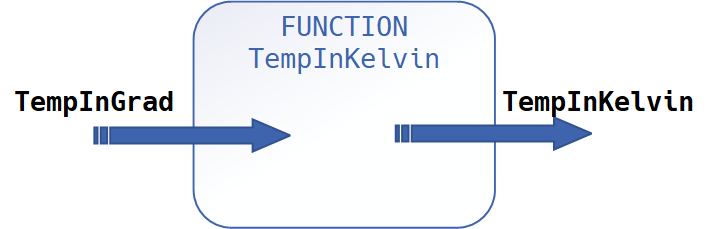
\includegraphics[width=0.7\textwidth]{bilder/FC_bild.png}}
				\caption{Konzept der Code-Kapselung der Temperaturumrechnung}
				\label{fig:fc_temp}
			\end{figure}

\pagebreak
\section{Lösung}
Nachfolgend ist der Code für die Umrechnung dargestellt.  
\bigskip

\scriptsize
\lstinputlisting[caption={Functionblock für Kelvinumrechnung},captionpos=b]{code/code.st}
    
\normalsize
\bigskip

Ich der Zeile 1 wird die Funktion deklariert und der Rückgabetyp der Funktion mit REAL festgelegt.  In den Zeilen 2 bis 7 werden die Eingangs- und lokalen Variablen deklariert.  Die Umrechnung der Eingangstemperatur von °C in K findet in Zeile 8 nach Formel \eqref{eq:kelvinumrechnung} statt.  Mit der Zeile 11 wird die Funktion abgeschlossen. 

\pagebreak

\section{Reflektion}
Hat Spass gemacht. 

\section{Quellen}

\printbibliography

\pagebreak

\section{Anhang}

Hilfreiche Links: 
\begin{itemize}[nosep]
	\item Formatierung Latex-Code: \url{https://c.albert-thompson.com/latex-pretty/}
	\item Tabellen in Latex 1: \url{https://www.tablesgenerator.com/}
	\item Tabellen in Latex 2: \url{https://github.com/krlmlr/Excel2LaTeX}
	\item Formeln in Latex: \url{https://www.codecogs.com/latex/eqneditor.php}
\end{itemize}

\bigskip

Update Literaturverzeichnis:
	 \begin{itemize}[nosep]
  				\item literatur.bib anpassen
  				\item Zitate einfügen
  				\item Dokument mit LaTeX kompilieren
  				\item in der Komandozeile im Ordner des Projektes "biber <<Projektname-Ohne-Endung>>" aufrufen
  				\item Dokument mit LaTex kompilieren 
	\end{itemize}

\pagebreak

\section{Anpassung auf Basis des Feedbacks}

Hier ist der Ort, wo Anpassungen aufgrund des Feedbacks des Betreuers beschrieben bzw. durchgeführt sind.


\end{document}